% -*- LaTeX -*- %%%%%%%%%%%%%%%%%%%%%%%%%%%%%%%%%%%%%%%%%%%%%%%%%%%%%%
%
% Template for scribing COMP163 - Computational Geometry 
%
% Spring, 2004
%
%%%%%%%%%%%%%%%%%%%%%%%%%%%%%%%%%%%%%%%%%%%%%%%%%%%%%%%%%%%%%%%%%%%%%%
%**start of header 

\documentclass [12pt]{article}
\usepackage{epsfig}
\usepackage{enumitem}
\usepackage{amsmath}
\usepackage[color, leftbars]{changebar}

\usepackage{caption}
\usepackage{subcaption}


\usepackage{color}
\definecolor{light-gray}{gray}{0.97} % shade of grey
\definecolor{dkgreen}{rgb}{0,0.6,0}
\definecolor{gray}{rgb}{0.5,0.5,0.5}
\definecolor{mauve}{rgb}{0.58,0,0.82}

%%%%%%%%%%%%%%%%%%%%%%%%%%%%%%%%%%%%%%%%%%%%%%%%%%%%%%%%%%%%%%%%%%%%%%%%
\usepackage{xcolor}
%% https://tex.stackexchange.com/questions/401750/quick-and-short-command-for-coloring-one-word
\newcommand\shorthandon{\catcode`@=\active \catcode`^=\active \catcode`*=\active }
\newcommand\shorthandoff{\catcode`@=12 \catcode`^=7 \catcode`*=12 }
\shorthandon
\def@#1@{\textcolor{red}{#1}}%
\def^#1^{\textcolor{blue}{#1}}%
\def*#1{\string#1}
\shorthandoff
%% useage: \textcolor{red}{text here}
% \shorthandon
% This is a @test@ of the ^emergency^ bro*@dcast system.
% \shorthandoff
%%%%%%%%%%%%%%%%%%%%%%%%%%%%%%%%%%%%%%%%%%%%%%%%%%%%%%%%%%%%%%%%%%%%%%%%


\setlength{\textwidth}{6.5in}
\setlength{\textheight}{9in}
\setlength{\oddsidemargin}{0in}
\setlength{\evensidemargin}{0in}
\setlength{\topmargin}{-0.5in}

\setlength{\parindent}{0pt}

\newtheorem{theorem}{Theorem}[section]
\newtheorem{definition}[theorem]{Definition}
\newtheorem{claim}[theorem]{Claim}
\newtheorem{lemma}[theorem]{Lemma}
\newtheorem{proof}[theorem]{Proof}

\newlength{\toppush}
\setlength{\toppush}{2\headheight}
\addtolength{\toppush}{\headsep}

\usepackage{hyperref}
\hypersetup{
    colorlinks=true,
    linkcolor=blue, % was previously black
    filecolor=magenta,
    urlcolor=blue,
    pdftitle={Template}
}
\urlstyle{same}

%\doheading{2}{title}{Last Revised: January, 2004}
%\htitle{title}

\def\subjnum{Comp 163}
\def\subjname{Computational Geometry}

\def\doheading#1#2#3{\vfill\eject\vspace*{-\toppush}%
  \vbox{\hbox to\textwidth{{\bf} \subjnum: \subjname \hfil Amy Bui}%
    \hbox to\textwidth{{\bf} Tufts University, Fall 2022 \hfil#3\strut}%
    \hrule}}

\newcommand{\htitle}[1]{\vspace*{3.25ex plus 1ex minus .2ex}%
\begin{center}
{\large\bf #1}
\end{center}} 

%%%%%%%%%%%%%%%%%%%%%%%%%%%%%%%%%%%%%%%%%%%%%%%%%%%%%%%%%%%%%%%%%%%

\begin{document}
\doheading{2}{title}{HW 4} 
% \htitle{Homework 1}
% \bigskip 
% \bigskip 
%%%%%%%%%% begin text after this line %%%%%%%%%%%%%%

    %%%%%%%%%%%%%%%%%%%%%%%%%%%%%%%%%%%%%%%%%%%%%%%%%%%%%%%%%%%%%%%%%%%%%%%%%
    \section{Delaunay Triangulation, Voronoi Diagram, and Gabriel Graph}
    \label{sec:one}

        % Relate the Delaunay triangulation and Voronoi diagram to edges that appear in the Gabriel Graph. (Hint: The Gabriel Graph is a subgraph of the Delaunay triangulation). Don't all edges of a Delaunay triangle cross a Voronoi edge? Prove it in both directions. \\

        Show that $p_i$ and $p_j$ have an edge in $\mathcal{GG}(S)$  if and only if $\overline{p_i p_j}$ appears in the $\mathcal{DT}(S)$ and $\overline{p_i p_j}$ crosses its dual Voronoi edge.\\

        ($\Rightarrow$) For two points $p_i, p_j \in S$, $\overline{p_i p_j}$ is the edge that connects them, and $C_{ij}$ is the circle with $\overline{p_i p_j}$ as the diameter. We say that $C_{ij}$ is an empty circle with no points of $S$ in its interior and therefore $\overline{p_i p_j} \in \mathcal{GG}(S)$; we then consider a third point $p_k\in S$, where $p_k \neq p_i, p_j$ and $p_k$ is not interior to $C_{ij}$. Point $p_k$ is either: 

        \begin{enumerate}
            \item $p_k$ is on the circumference of $C_{ij}$. Therefore, by definition\footnote{Theorem 9.6.i \cite{berg08} pg. 198}, $\Delta p_i p_j p_k$ is a face in the Delaunay triangulation, and so $\overline{p_i p_j} \in \mathcal{DT}(S)$ (as do the other edges formed by the three points). $\Delta p_i p_j p_k$ is a right triangle because they are three points on a circle whose diameter is the hypotenuse. The Voronoi vertex that is the end point of the dividing Voronoi edge between $p_i$ and $p_j$ must be located within the right triangle, equidistance from the three points, and the edge must intersect the circumcenter given by the midpoint of $\overline{p_i p_j}$, because there are no other points intertior or on the circle for which more Voronoi edges would form.
            \item $p_k$ is exterior to $C_{ij}$. Therefore, by definition\footnote{Theorem 9.6.ii \cite{berg08} pg. 198}, $\overline{p_i p_j} \in \mathcal{DT}(S)$ and the $\overline{p_i p_j}$ could only cross the dividing Voronoi edge that separates the regions of site $p_i$ and $p_j$.
        \end{enumerate}

        ($\Leftarrow$) Given $\overline{p_i p_j}$ appears in the $\mathcal{DT}(S)$ and $\overline{p_i p_j}$ crosses its dual Voronoi edge, I show by contradiction that $\overline{p_i p_j}$ is also in the $\mathcal{GG}(S)$\footnote{Jake}. \\

        Suppose that $\overline{p_i p_j}$ doesn't cross its dual Voronoi edge. This means that the dividing edge was ``pushed'' either above or below $\overline{p_i p_j}$, and $\overline{p_i p_j}$ now intersects two other edges of a third Voronoi cell, given by $p_k$. So there is a Voronoi vertex equidistance from the three points and this vertex and the edge it's on doesn't intersect the midpoint of $\overline{p_i p_j}$. This position means the distance between $p_i$ and $p_k$, and the distance between $p_j$ and $p_k$ are both shorter than the distance between $p_i$ and $p_j$. Therefore, taking the circle with the diameter $\overline{p_i p_j}$, $p_k$ must lie interior to the circle. Therefore, $\overline{p_i p_j}$ cannot be in  $\mathcal{GG}(S)$. (Note that this edge can still be in $\mathcal{DT}(S)$ if the circle given by $\Delta p_i p_j p_k$ have no interior points; this just simply means that $\overline{p_i p_j}$ doesn't pass through its circumcircle).\\

        % The $\mathcal{DT}(S)$ is the dual of the $\mathcal{VD}(S)$; by definition, the vertices of $\mathcal{DT}(S)$ are Voronoi sites and the edges of $\mathcal{VD}(S)$ are those that connect those circumcenters in $\mathcal{DT}(S)$ that share a triangle edge (and so, cross that edge). We can conclude that for $\overline{p_i p_j} \in \mathcal{GG}(S)$ if and only if $\overline{p_i p_j} \in \mathcal{DT}(S)$, because $\mathcal{GG}(S)\subseteq \mathcal{DT}(S)$. \\




        Since $\mathcal{GG}(S)\subseteq \mathcal{DT}(S)$, we can find $\mathcal{GG}(S)$ very easily. First, compute the $\mathcal{DT}(S)$, which can be done in $O(n\log n)$ time and $O(n)$ space\footnote{Theorem 9.12 \cite{berg08} pg. 206}. Then, We can walk the edges of $\mathcal{DT}(S)$ in $O(n)$ time, and check each if the circle with just that edge, $\overline{p_i p_j}$, as the diameter contains an interior point or not. Since this was an edge in the $\mathcal{DT}$, there is only one potential point that could be interior, the third point in the triangle; so we only need to check if the neighbors of $p_i, p_j$ are interior to $C_{ij}$; assuming general position, there is a constant number of neighbors to check, 2 for each point. If it has interior points, then discard that edge; otherwise, it is an edge in $\mathcal{GG}(S)$. The total runtime is $O(n\log n)$ due to computing the $\mathcal{DT}(S)$, which is optimal and faster than checking every pair of points with every other point for being interior, which would come out to be $O(n^3)$ time.

        


        % \begin{enumerate}[label=\alph*.]
        %     \item 
        % \end{enumerate}
        
    \pagebreak
    % END %%%%%%%%%%%%%%%%%%%%%%%%%%%%%%%%%%%%%%%%%%%%%%%%%%%%%%%%%%%%%%%%%%%

    
    %%%%%%%%%%%%%%%%%%%%%%%%%%%%%%%%%%%%%%%%%%%%%%%%%%%%%%%%%%%%%%%%%%%%%%%%%
    \section{Voronoi Diagrams in $L_1$ and $L_\infty$ Metrics}
    \label{sec:two}

    % Reference: \cite{leewong}, \cite{voronoiinteract}

    I use the the grid layout in MS powerpoint (grid lines don't export) to draw the below diagrams. The Voronoi diagram in the $L_1$ metric is given in solid \textcolor{red}{red} lines; it is made of the bisectors (\textcolor{red}{$B_1$'s}) that separate the regions of two separate points. The Voronoi diagram in the $L_\infty$ metric is given in solid \textcolor{dkgreen}{green} lines; it is made of the bisectors (\textcolor{dkgreen}{$B_\infty$'s}) that separate the regions of two separate points. The regular Voronoi diagram (given in the $L_2$ metric) is given in the thicker dashed \textcolor{blue}{blue} lines (the segment connecting two points is thin-dashed); it is made of the perpendicular bisectors (\textcolor{blue}{$B_2$'s}) that separate the regions of two separate points. \\
    
    I start by characterizing the bisectors between two points $q_i(x_i, y_i)$ and $q_j(x_j, y_j)$ in the three different metrices in different general positions using real values for points; $q_i$ will be left of $q_j$, i.e. $x_i < x_j$; everything to one side of a bisector $B_p$ in the $L_p$ metric is closer to one point than it is so the other, because the bisectors are equal distance from either points. $L_1$-distance is $d_1 (q_i, q_j) = |x_i - x_j| + |y_i - y_j|$; $L_\infty$-distance is $d_\infty (q_i, q_j) = \text{max}\Big(|x_i - x_j|,\ |y_i - y_j| \Big) $\footnote{Jake}. Points on the bisectors are found by taking half of the distance. \\
    
    In each of the six cases below, notice that $B_2$ is bounded by $B_1$ and $B_\infty$ which have a criss-cross pattern with each other\cite{leewong}. In general, for $1 \leq p \leq \infty$, we can say that $B_p$ is bounded by $B_1$ and $B_\infty$, and that all dividing edges in each metrices intersect at a common point in the rectangle given by $q_i$ and $q_j$. In the case that $q_i$ and $q_j$ form a square region (when $|x_i - x_j| = |y_i - y_j|$), there are two regions in the $L_1$ metric shaded in red in which any point there could be equal distance from $q_i$ and $q_j$; for the diagrams below, I take the bisector in the dark, solid red; likewise for the bisector shown for the $L_\infty$ metric. 

    \begin{figure}[h]
        \begin{tabular}{cc}
            \begin{subfigure}{0.5\textwidth}
                \centering
                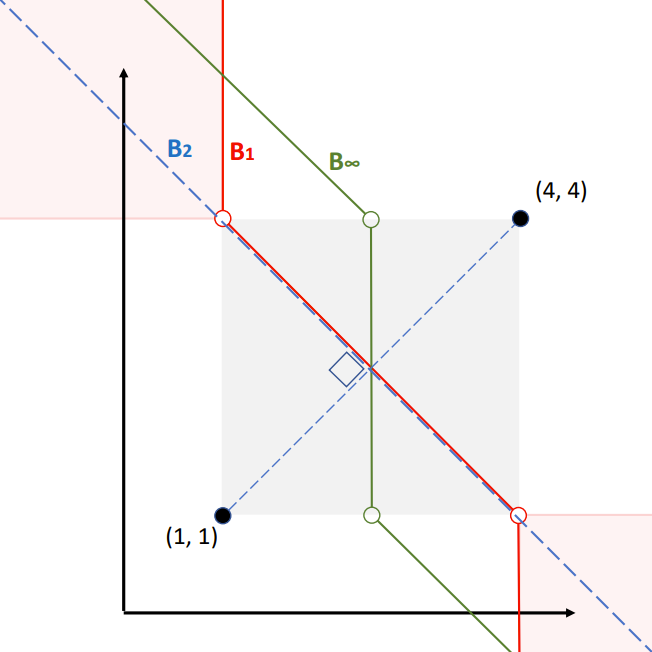
\includegraphics[width=1\textwidth]{images/2e.PNG}
                \caption{$|x_i - x_j| = |y_i - y_j|$, $y_i < y_j$}
                \label{fig.2e}
            \end{subfigure} & 
            \begin{subfigure}{0.5\textwidth}
                \centering
                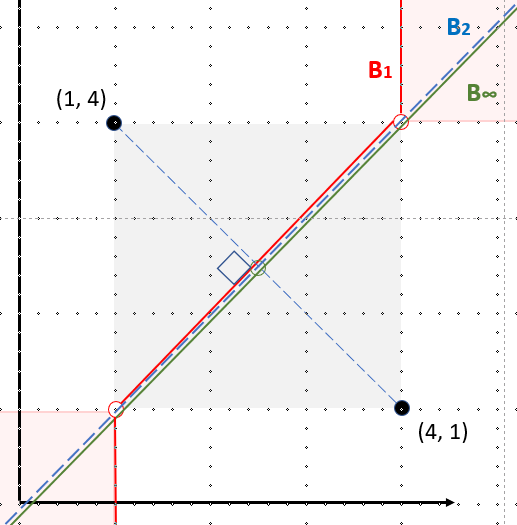
\includegraphics[width=1\textwidth]{images/2f.PNG}
                \caption{$|x_i - x_j| = |y_i - y_j|$, $y_i > y_j$}
                \label{fig.2f}
            \end{subfigure}
        \end{tabular}
        % \caption{When $|x_i - x_j| = |y_i - y_j|$ (square)}
        \label{fig.2e2f}
    \end{figure}

    \pagebreak

    \begin{figure}[h]
        \begin{tabular}{cc}
            \begin{subfigure}{0.5\textwidth}
                \centering
                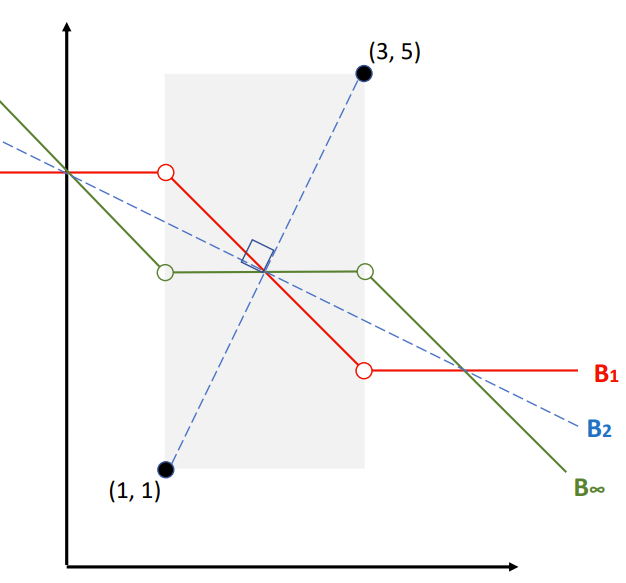
\includegraphics[width=1\textwidth]{images/2a.PNG}
                \caption{$|y_i - y_j| > |x_i - x_j|$, $y_i < y_j$}
                \label{fig.2a}
            \end{subfigure} & 
            \begin{subfigure}{0.5\textwidth}
                \centering
                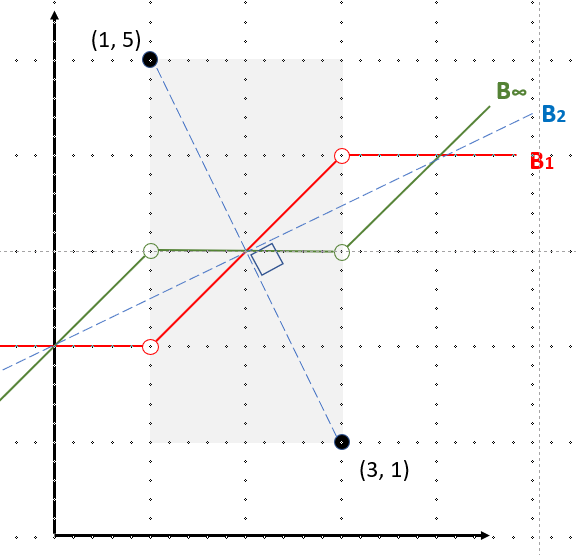
\includegraphics[width=1\textwidth]{images/2b.PNG}
                \caption{$|y_i - y_j| > |x_i - x_j|$, $y_i > y_j$}
                \label{fig.2b}
            \end{subfigure} \\
            \begin{subfigure}{0.5\textwidth}
                \centering
                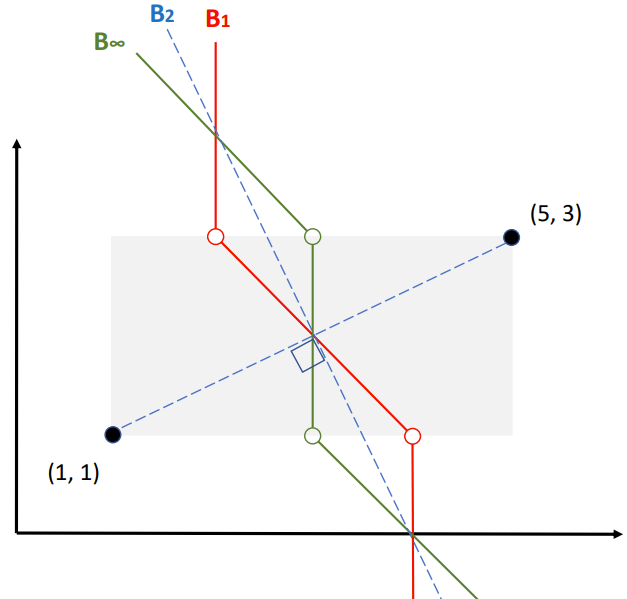
\includegraphics[width=1\textwidth]{images/2c.PNG}
                \caption{$|x_i - x_j| > |y_i - y_j|$, $y_i < y_j$}
                \label{fig.2c}
            \end{subfigure} & 
            \begin{subfigure}{0.5\textwidth}
                \centering
                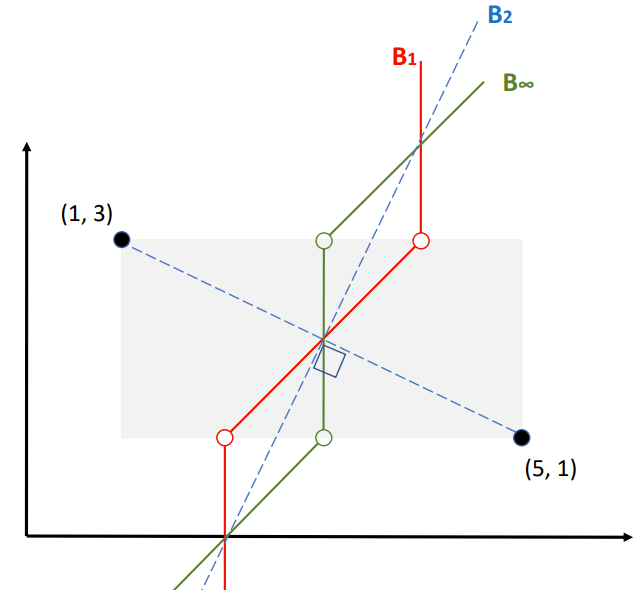
\includegraphics[width=1\textwidth]{images/2d.PNG}
                \caption{$|x_i - x_j| > |y_i - y_j|$, $y_i > y_j$}
                \label{fig.2d}
            \end{subfigure}
        \end{tabular}
        % \caption{When $|y_i - y_j| > |x_i - x_j|$}
        \label{fig.2a2b}
    \end{figure}

    % \pagebreak

    % \begin{figure}[h]
    %     \begin{tabular}{cc}
    %         \begin{subfigure}{0.5\textwidth}
    %             \centering
    %             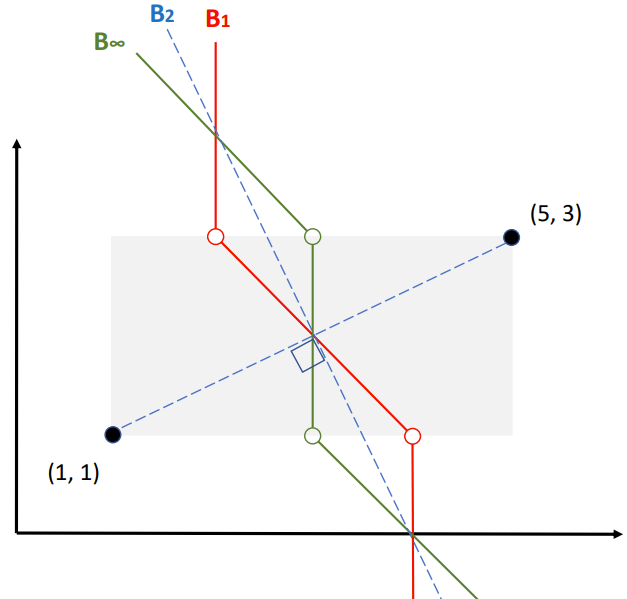
\includegraphics[width=1\textwidth]{images/2c.PNG}
    %             \caption{$y_i < y_j$}
    %             \label{fig.2c}
    %         \end{subfigure} & 
    %         \begin{subfigure}{0.5\textwidth}
    %             \centering
    %             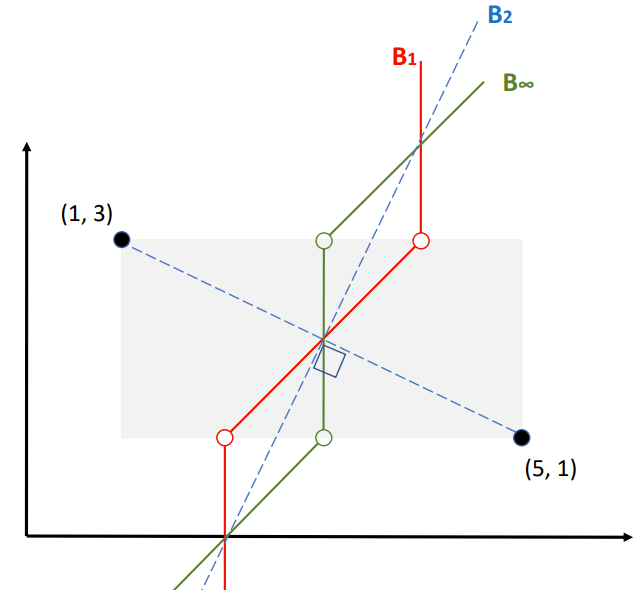
\includegraphics[width=1\textwidth]{images/2d.PNG}
    %             \caption{$y_i > y_j$}
    %             \label{fig.2d}
    %         \end{subfigure}
    %     \end{tabular}
    %     \caption{When $|x_i - x_j| > |y_i - y_j|$}
    %     \label{fig.2c2d}
    % \end{figure} 


    

    \pagebreak



    % In an arbitrary $d$-dimensional plane $R^d$, for a real number $1 \leq p \leq \infty$, the $L_p$-distance between two points $q_i(x_{i1}, x_{i2}, ... x_{id})$ and $q_j(x_{j1}, x_{j2}, ... x_{jd})$ is given by the norm: $$ d_{p}(q_i, q_j) = \Big[ \sum_{k = 1}^{d} \Big( |x_k(q_i) - x_k(q_j)| \Big) \Big]^{\frac{1}{p}} $$

    % The plane in which the $L-p$ distance is measured is denoted $R^d_p$. \\


    % In a 2D plane $R^{2}$, given two points $q_i(x_i, y_i)$ and $q_j(x_j, y_j)$, the distance between them in the $L_1$ metric ($R^2_1$ plane) is given by: $$ d_{1}(q_i, q_j) = |x_i - x_j| + |y_i - y_j| $$

    % The distance between them in the $L_\infty$ metric ($R^2_\infty$ plane) is given by: $$ d_{\infty}(q_i, q_j) = \text{max}\Big( |x_i - x_j|, |y_i - y_j| \Big)  $$


    % There exists a linear mapping $f$ from the $R^2_\infty$ plane to the $R^2_1$ plane. For a point $(x, y) \in R^2_\infty$, there exists a point $(x', y') \in R^2_1$ where $x' = \frac{y + x}{2}$ and $y' = \frac{y - x}{2}$. The distance between two points $q_i, q_j \in R^2_\infty$ is equal to the distance between their images $q_i', q_j' \in R^2_1$. \\

    % For example, let $q_i(x_i, y_i), q_j(x_j, y_j) \in R^2_\infty$ and let $x_j > x_i$, $y_i > y_j$, and $y_j - y_i > x_j - x_i$. So the between them is $d_{\infty}(q_i, q_j) =  y_j - y_i $.\\ 

    % The distance between $q_i'(x_i', y_i'), q_j'(x_j', y_j') \in R^2_1$ is equal to $d_{\infty}(q_i, q_j)$: 

    % \begin{align*}
    %     d_{1}(q_i', q_j')   &= |x_j' - x_i'| + |y_j' - y_i'| \\ 
    %                         &= \Big( \frac{y_j + x_j}{2} - \frac{y_i + x_i}{2} \Big) + \Big( \frac{y_j - x_j}{2} - \frac{y_i - x_i}{2} \Big) \\ 
    %                         &= \frac{1}{2} \Big( (y_j - y_i) + (x_j - x_i) \Big) + \frac{1}{2} \Big( (y_j - y_i) - (x_j - x_i) \Big)\\ 
    %                         &= \frac{1}{2} \Big( 2(y_i - y_j) + (x_j - x_i) - (x_j - x_i) \Big) \\
    %                         &= y_i - y_j \\ 
    %                         &= d_{\infty}(q_i, q_j)
    % \end{align*}




    \begin{enumerate}[label=(\alph*)]
        \setcounter{enumi}{0}
        \item \textbf{Voronoi Diagram in $L_1$ Metric}
    \end{enumerate}

        \begin{figure}[h]
            \centering
            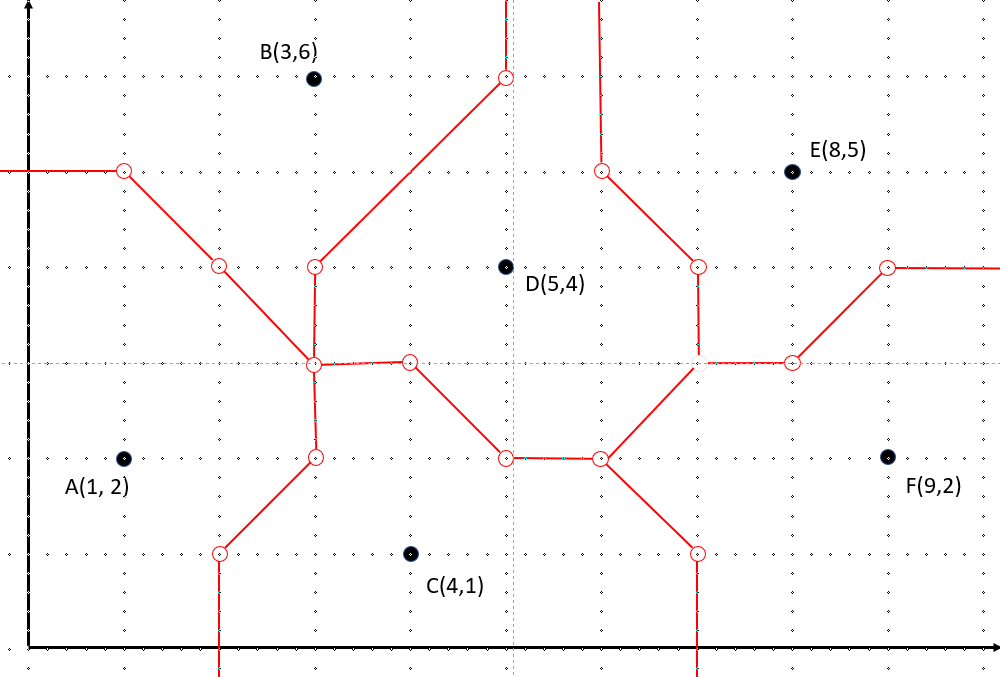
\includegraphics[width=1\textwidth]{images/L1plain.PNG}
            \caption{$L_1$ metric Voronoi diagram for a set of 6 points using the $L_1$-distance formula above. Fig. \ref{fig.L1detailed} is a detailed version that extends the bisectors of pairs of points. See Fig. \ref{fig.LINFplain} for the $L_\infty$ Voronoi diagram for these points, and Fig. \ref{fig.L1LINFplain} for the two overlayed.}
            \label{fig.L1plain}
        \end{figure}

    \pagebreak


    \begin{enumerate}[label=(\alph*)]
        \setcounter{enumi}{1}
        \item \textbf{Voronoi Diagram in $L_\infty$ Metric}
    \end{enumerate}

        \begin{figure}[h]
            \centering
            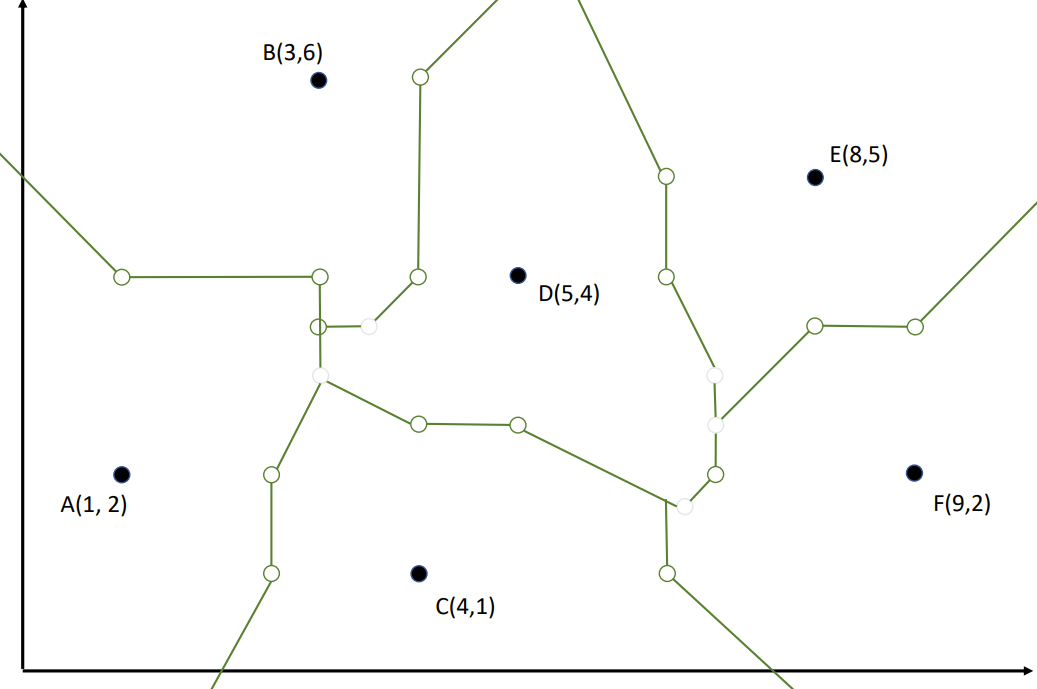
\includegraphics[width=1\textwidth]{images/LINFplain.PNG}
            \caption{$L_\infty$ metric Voronoi diagram for the same set of 6 points above using the $L_\infty$-distance formula. Fig. \ref{fig.LINFdetailed} is a detailed version that extends the bisectors of pairs of points. See Fig. \ref{fig.L1plain} for the $L_1$ Voronoi diagram for these points, and Fig. \ref{fig.L1LINFplain} for the two overlayed.}
            \label{fig.LINFplain}
        \end{figure}

    \pagebreak



    \begin{enumerate}[label=(\alph*)]
        \setcounter{enumi}{2}
        \item \textbf{Voronoi Diagrams of the $L_1$ and $L_\infty$ Metric}
    \end{enumerate}

        \begin{figure}[h]
            \centering
            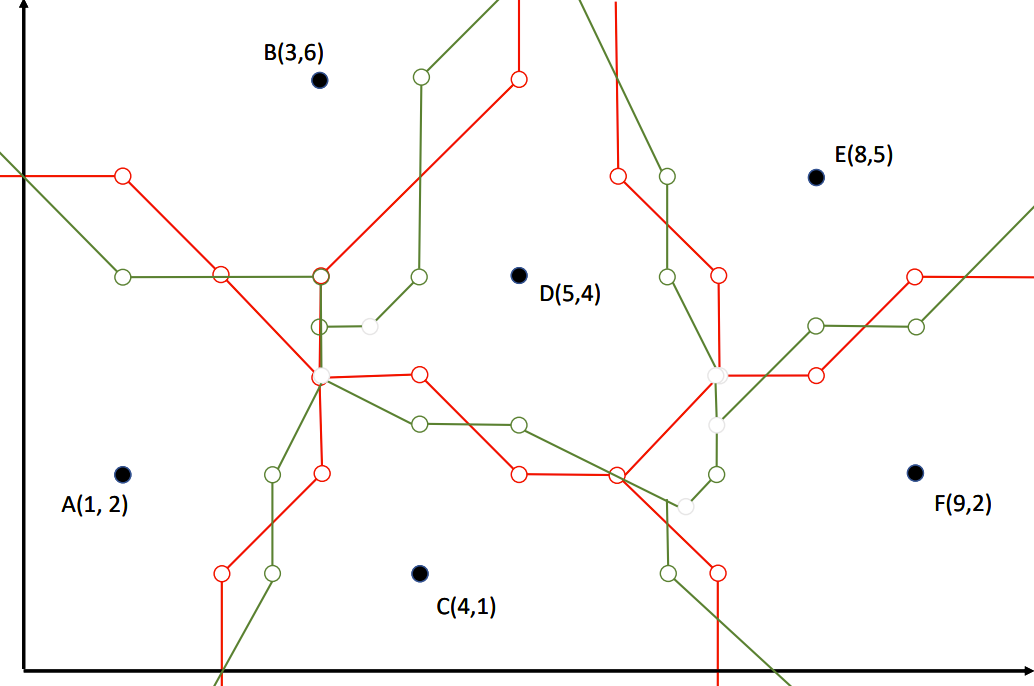
\includegraphics[width=1\textwidth]{images/L1LINFplain.PNG}
            \caption{This overlay of the $L_1$ and $L_\infty$ Voronoi diagrams shows the same criss-cross patterns seen and described above in Fig. \ref{fig.2e} - \ref{fig.2d}, when we overlay the $B_1(q_i, q_j)$ and $B_\infty(q_i, q_j)$ for two given points in the plane. I expect the corresponding $L_2$ Voronoi diagram to be contained in the bounds of these two diagrams. See. Fig. \ref{fig.L1LINFL2arrow}, where the $L_2$ Voronoi diagram (Fig. \ref{fig.L2}) is overlayed.}
            \label{fig.L1LINFplain}
        \end{figure}

        \pagebreak


        \begin{figure}[h]
            \centering
            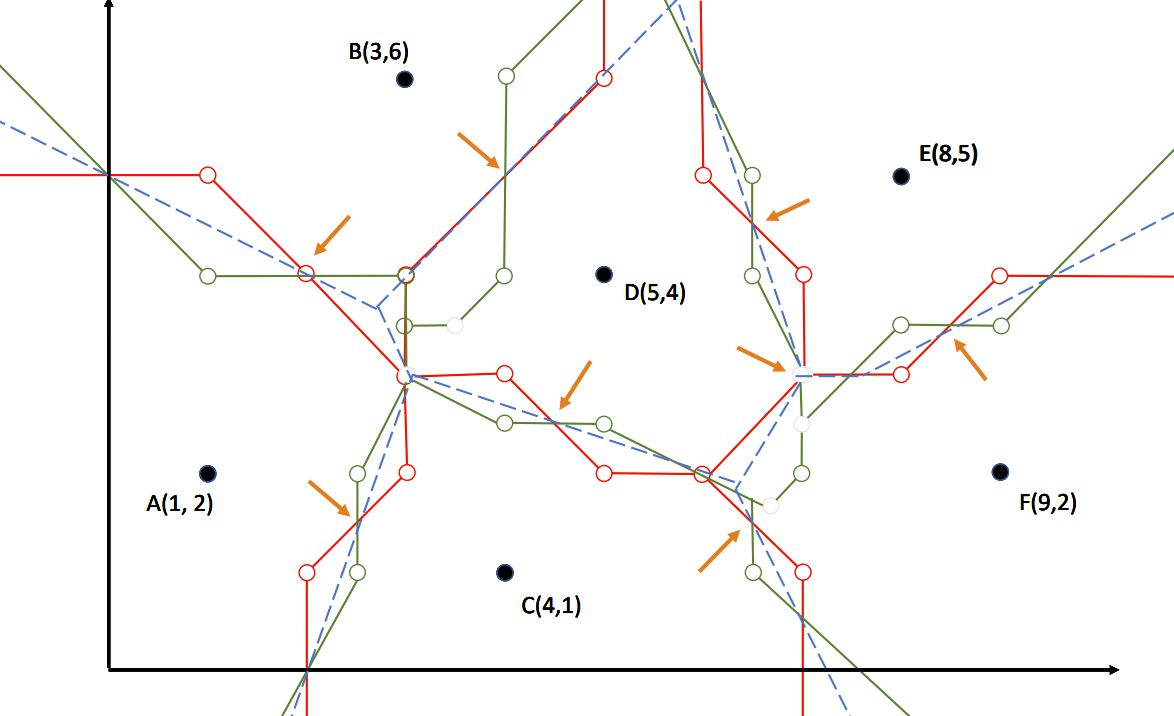
\includegraphics[width=1\textwidth]{images/L1LINFL2arrow.PNG}
            \caption{An overlay of the $L_1$, $L_2$, $L_\infty$ Voronoi diagrams. We see the blue dashed edges of the $L_2$ diagram within the bounds of the edges of the $L_1$ and $L_\infty$ diagrams. The orange arrows point to where three edges of the three diagrams intersect at the mid-point of a segment $\overline{q_i q_j}$. See Fig. \ref{fig.L2} for just the $L_2$ Voronoi diagram.}
            \label{fig.L1LINFL2arrow}
        \end{figure} 


        
    \pagebreak
    % END %%%%%%%%%%%%%%%%%%%%%%%%%%%%%%%%%%%%%%%%%%%%%%%%%%%%%%%%%%%%%%%%%%%



    %%%%%%%%%%%%%%%%%%%%%%%%%%%%%%%%%%%%%%%%%%%%%%%%%%%%%%%%%%%%%%%%%%%%%%%%%
    \section{Points in a Diagram}
    \label{sec:three}

    \begin{enumerate}[label=\alph*.] 
        \item We assume general position of $S$ and that we've already computed the Voronoi Diagram for $S$, $\mathcal{VD}(S)$, which takes $O(n\log n)$ time, and that the edges, vertices, and faces of $\mathcal{VD}(S)$ are stored in a DCEL. We can do point location on $q$ in $O(\log n)$ time to detect which Voronoi cell it is in. Since this is a Voronoi Diagram, whatever face query point $q$ is in, the Voronoi site, point $p\in S$, to which the current face/cell belongs, will be the closest point to $q$, because $q$ is in a region in which it is closer to $p\in S$ than it is to any other point $r\in S$, $r \neq p$. Therefore, using $q(x_q, y_q)$ and closest point $p(x_p, y_p)$, we can calculate in consant time the largest radius circle $C_q$ can have without including $p$ using the distance formula, $r = \sqrt{|x_q - x_p|^2 + |y_q - y_p|^2} - \epsilon$; finally, we can report the largest circle centered at $q$ for the problem, $C_q = (x - x_q)^2 + (y - y_q)^2 = r^2$. Space complexity is linear because we are storing the diagram in a DCEL. Overall runtime if we don't have to compute the $\mathcal{VD}(S)$ is $O(\log n)$ for one query point in order to do point location. For $m$ query points, the total runtime is $O(m \log n)$.
        

        \item Again, assume general position and that both $\mathcal{CH}(S)$ and $\mathcal{VD}(S)$ are computed (each takes $O(n\log n)$ time), overlayed, and their edges added to the same DCEL. We remove the partial edges $\mathcal{VD}(S)$ that are outside $\mathcal{CH}(S)$, since the path must be contained within the hull; we can walk the edges of the $\mathcal{CH}(S)$ to find the intersection points with edges of $\mathcal{VD}(S)$ and remove those beyond the hull. This takes $O(n\log n)$ time. 
        
        To find a path from $p$ to $q$, the ``safest'' possible path would be some route that is as far from any points in $S$ as possible. This describes the edges of the $\mathcal{VD}(S)$, because points of the edges are halfway between two given sites, and are therefore the furthest possible points from two points in $S$. This does not necessarily mean all edges are ``safe'' to walk, i.e. $> k$ distance from a site\footnote{Diane discussed with us possible ways to find a path that met the k-tolerance condition, including walking on the Voronoi edges and how to tackle it from the Piano Mover's problem perspective.}.

        So then, for each point $t\in S$, we create a circle centered at $t$ with radius $k$. For every partial edge that intersects the circles and are contained in the circle, remove those partial edges from the DCEL, as well. This can be done in $O(n\log n)$ time. We are now left with a DCEL, with possibly disjointed subgraphs, but with edges and vertices that are $> k$ distance away from a site in $S$. 
        
        From both $p$ and $q$, each creates a list of the nearest Voronoi edge or vertex to them, which, as stated, will be $> k$ distance from a Voronoi site. Then, using depth-first search, we calculate a path from $p$ to $q$ (or vice versa) (DFS is linear runtime). Report the result of the first successful DFS if a path is found; otherwise, a path that met the conditions did not exist and we report no path. 

        Finally, overall space complexity is linear for the DCEL. 
    \end{enumerate}


    \pagebreak
    % END %%%%%%%%%%%%%%%%%%%%%%%%%%%%%%%%%%%%%%%%%%%%%%%%%%%%%%%%%%%%%%%%%%%



    %%%%%%%%%%%%%%%%%%%%%%%%%%%%%%%%%%%%%%%%%%%%%%%%%%%%%%%%%%%%%%%%%%%%%%%%%
    \section{Project}
    \label{sec:four}

    
    
        
    \pagebreak
    % END %%%%%%%%%%%%%%%%%%%%%%%%%%%%%%%%%%%%%%%%%%%%%%%%%%%%%%%%%%%%%%%%%%%


    %%%%%%%%%%%%%%%%%%%%%%%%%%%%%%%%%%%%%%%%%%%%%%%%%%%%%%%%%%%%%%%%%%%%%%%%%
    \section{Appendix}
    \label{sec:five}

    The below figures are the detailed versions of previous figures in problem 2. The faded out portion of the diagrams are the bisectors dividing regions of different pairs of points that are not part of the final voronoi diagrams. The faded colored letters indicate which half plane belonged to which region, and the faded grey letters are those half planes of the individual bisectors not in the final diagrams. 
    
    \begin{figure}[h]
        \centering
        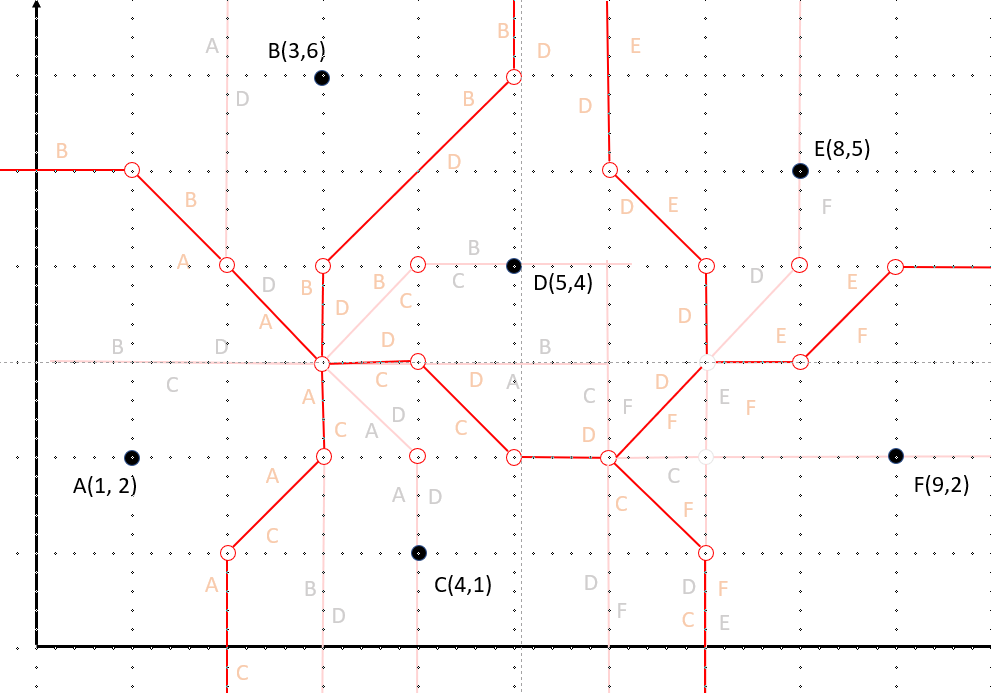
\includegraphics[width=1\textwidth]{images/L1detailed.PNG}
        \caption{Detailed version of $L_1$ metric Voronoi Diagram of Fig. \ref{fig.L1plain}}
        \label{fig.L1detailed}
    \end{figure}

    \begin{figure}[h]
        \centering
        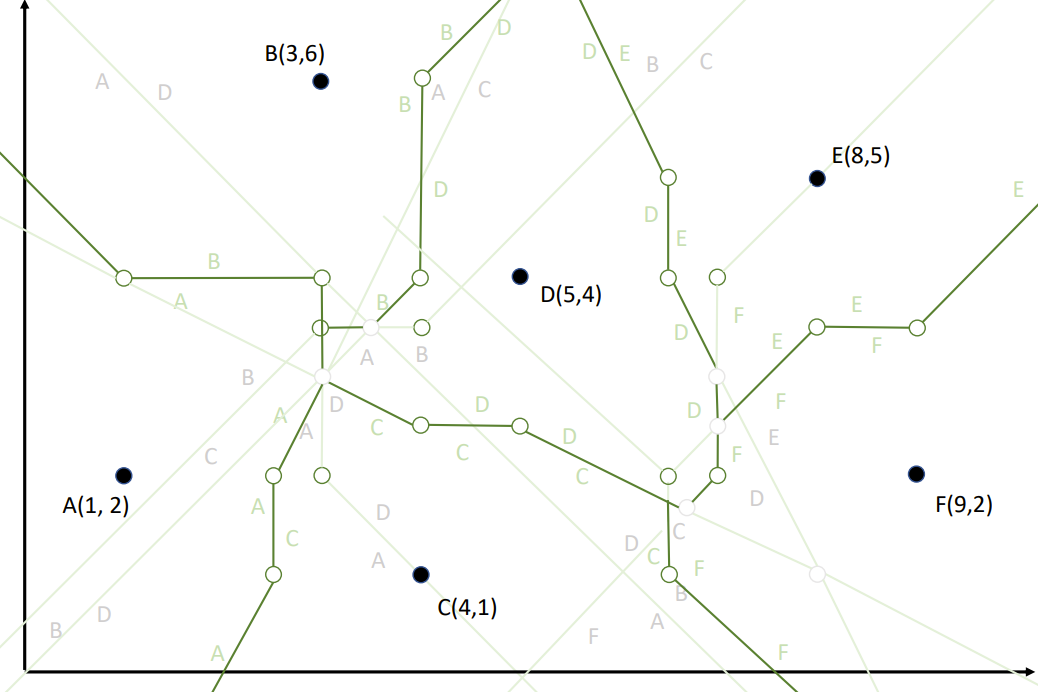
\includegraphics[width=1\textwidth]{images/LINFdetailed.PNG}
        \caption{Detailed version of $L_\infty$ metric Voronoi Diagram of Fig. \ref{fig.LINFplain}}
        \label{fig.LINFdetailed}
    \end{figure}
    \pagebreak


    
    \begin{figure}[h]
        \centering
        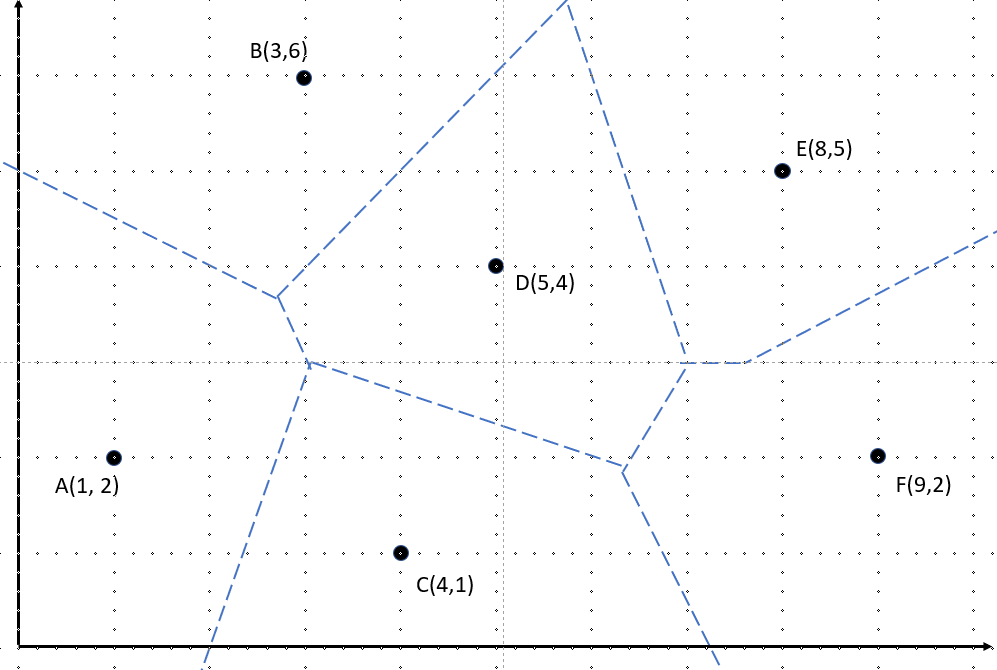
\includegraphics[width=1\textwidth]{images/L2.PNG}
        \caption{The $L_2$ Voronoi diagram for the 6 points examined in problem 2.}
        \label{fig.L2}
    \end{figure}

    \pagebreak
    % END %%%%%%%%%%%%%%%%%%%%%%%%%%%%%%%%%%%%%%%%%%%%%%%%%%%%%%%%%%%%%%%%%%%





    %%%%%%%%%%%%%%%%%%%%%%%%%%%%%%%%%%%%%%%%%%%%%%%%%%%%%%%%%%%%%%%%%%%%%%%%%
    

    % \pagebreak
    % END %%%%%%%%%%%%%%%%%%%%%%%%%%%%%%%%%%%%%%%%%%%%%%%%%%%%%%%%%%%%%%%%%%%



\begin{thebibliography}{1}
    \bibitem[1]{officehours}Jake and Diane's office hours, classmates: Stephanie, Alex, Anju with homework problem discussions.
    \bibitem[2]{berg08}Mark de Berg, Otfried Cheong, Marc van Kreveld, and Mark Overmars. 2008. Computational Geometry: Algorithms and Applications (3rd ed. ed.). Springer-Verlag TELOS, Santa Clara, CA, USA.
    \bibitem[3]{leewong}D.T Lee and C.K. Wong, \href{https://epubs.siam.org/doi/epdf/10.1137/0209017}{``Voronoi Diagrams in $L_1$ and ($L_{\infty}$) Metrics with 2-Dimentional Storage Applications''}. SIAM J Comput. Vol. 9, No. 1, 200-212. 1980.
    \bibitem[4]{voronoiinteract}Yunzhi Shi, \href{http://yunzhishi.github.io/voronoi.html}{``Sarah's Interactive Voronoi Diagram''}. 2017.
\end{thebibliography}
%%%%%%%%%%%%%%%%%%%%%%%%%%%%%%%%%%%%%%%%%%%%%%%%%%%%%%%%%%%%%%%%%%%%%%
\end{document}
%%%%%%%%%%%%%%%%%%%%%%%%%%%%%%%%%%%%%%%%%%%%%%%%%%%%%%%%%%%%%%%%%%%%%%

